% Cheminformatics (4 weeks)

Chemical informatics is the branch of chemistry that attempts to solve chemical problems algorithmically on the computer, such as predicting reactivity based on substructure search or quantum chemical DFT calculations. \emph{RDKit} has become particularly established for this. It is an open-source based cheminformatics toolkit written in C++, but can also be used with Python, Java or JavaScript. Among other things, it includes the following functionalities:

\begin{itemize}
    \item Reading and writing of molecules
    \item Working with molecules in 2D and 3D
    \item Drawing 2D depictions
    \item Substructure search
    \item Chemical transformations
    \item Maximum common substructure
    \item Fingerprints and molecular similarity
    \item Descriptor calculation
    \item Chemical reactions
    \item Chemical features and pharmacophores
\end{itemize}

A central and fundamental area of cheminformatics is the digital \emph{representation of molecules}. For this, we had already introduced graph theory, whereby a molecule can be represented as a graph (vertices are the atoms and edges and their weight are the bonds as well as their bond multiplicity) using an adjacency list or adjacency matrix. Additional information, such as element, stereochemistry, charge or aromaticity, can also be stored in the vertex. The problem with this representation is that it is not very efficient for storage and molecules are difficult to compare. The standard file format for saving chemical structures with coordinates (from crystal structures) is, however, the \emph{Molefile} format, which works with a connection table and is shown below.

\begin{center}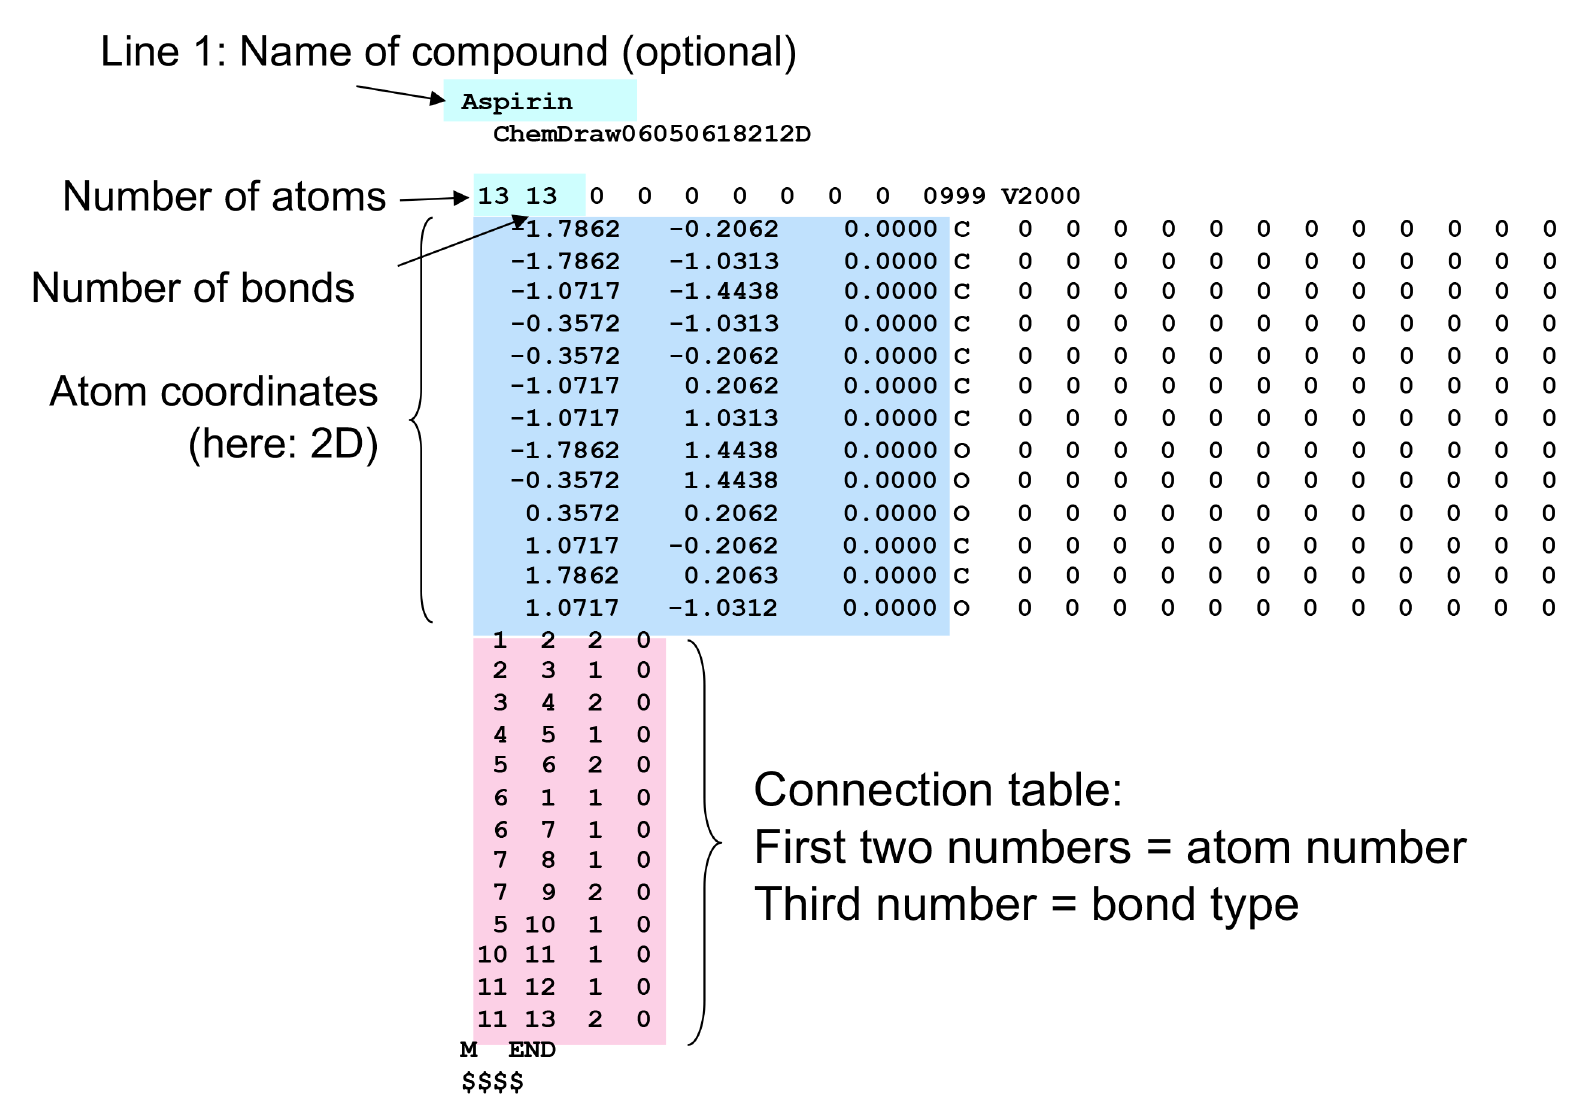
\includegraphics[width=0.85\textwidth]{img/cheminformatics/DataFormat.png}\end{center}

\subsection{1D representation}



\subsubsection{SMILES}

\subsubsection{Canonicalization}

\subsubsection{InChI}

\subsubsection{Ring perception}

\subsubsection{Aromaticity detection}

\subsection{Substructure search}

\subsubsection{SMARTS}

\subsubsection{Subgraph isomorphism}

\subsection{Chemical reactions}

\subsection{Dimensionality reduction}

\subsection{Fingerprints}

\subsection{Maximum common substructure}

\subsection{Scaffolds}

\subsection{Generation of 3D coordinates}

\subsubsection{Distance geometry}

\subsection{Clustering}

\subsubsection{Hierarchical}

\subsubsection{Application to chemical space}

\subsubsection{Non-hierarchical}

\subsubsection{Application to conformations}